\chapter{Robot RCM for Percutaneous Needle Interventions} \label{chap:chap-2}

\section{Chapter Overview}
\label{sec:chap-2-overview}

The current chapter is based on

\parencite{wangSafeSituNeedle2021}: Wang, Y., Li, G., Kwok, K., Cleary, K., Taylor, R. H., \& Iordachita, I. (2021). Towards Safe In Situ Needle Manipulation for Robot Assisted Lumbar Injection in Interventional MRI. Proceedings of the IEEE/RSJ International Conference on Intelligent Robots and Systems. IEEE/RSJ International Conference on Intelligent Robots and  Systems, 2021, 1835–1842.

\section{Introduction}
\label{sec:chap-2-introduction}

Needle insertion is often a necessary step in minimally invasive procedures, during which a hypodermic needle is inserted into the human body for diagnosis or treatment. One such application is lumbar injection therapy, in which a needle is guided into the lumbar spinal region, such as facet joints or the epidural space, and medication is injected to provide further diagnosis or give immediate pain relief. During the procedure, the physician advances a spinal needle and injects diagnostic or therapeutic agent once the needle reaches the anatomical target~\parencite{silbergleitImagingguidedInjectionTechniques2001}. Intraoperative imaging, such as fluoroscopy and computed tomography (CT), is routinely used as visual feedback to the physician due to their wide availability; however, ionizing radiation exposure puts both the patients and the physicians at higher risk of developing cancer, albeit the presence of dose-reducing measures~\parencite{giordanoCervicalSpineImaging2008,leeMeasurementsSurgeonsExposure2012}. Spinal needles are typically made from stainless steel and are sized with diameter of 18 gauge (1.02mm) or smaller~\parencite{silbergleitImagingguidedInjectionTechniques2001,calthorpeHistorySpinalNeedles2004,tsenNeedlesUsedSpinal2006}, making them flexible and subject to shape deformation.

Many spinal injection procedures require targeting of submillimeter nerves and thin anatomical spaces. Common targets are often surrounded by vulnerable structures such as major arteries and veins, increasing the chance of complications due to needle misplacement~\parencite{bogdukComplicationsSpinalDiagnostic2008}. Difficulties in accessing and visualizing these regions of human body necessitate the highest spatial and contrast image resolution and image guidance accuracy to ensure accurate and safe drug delivery, which is best provided by magnetic resonance imaging (MRI).

The idea of robot-assisted needle insertions under imaging guidance has been explored since early 2000s, and plenty of systems have been developed that can operate within the MR environment. For instance, Susil et al. developed an MR-compatible transrectal system to perform MRI-guided prostate biopsy procedures~\parencite{susilSystemMRImage2003,susilSystemProstateBrachytherapy2004}, and the device was further improved by Krieger et al.~\parencite{kriegerDesignNovelMRI2005}. This remotely actuated manipulator was able to place the needle tip to less than 2.3 mm from the target. Fischer et al. developed a pneumatically actuated needle placement device for real-time MRI-guided  transperineal prostate interventions~\parencite{fischerMRICompatiblePneumaticRobot2008}. Patel et al. designed a patient-mounted, 4 degree-of-freedom (DOF) robot actuated by piezoelectric motors for MRI-guided shoulder arthrography~\parencite{patelRoboticSystemMRIGuided2018}. Wu et al. designed a remotely actuated needle driving device that allows clinician to manually steer and insert the needle away from the scanner bore~\parencite{wuRemotelyActuatedNeedle2019}, and is incorporated into a 6-DOF robot for MRI-guided low back pain injection procedures~\parencite{liFullyActuatedBodyMounted2020a}.

Among these MR-compatible robotic systems, there are a few that have deliberate kinematic constraints to limit the robot motions in order to achieve a specific motion trajectory. Stoianovici et al. developed an MR-Safe robotic system that employs a parallelogram-type mechanism to physically enforce an RCM below the needle guide, and was able to achieve high structural stiffness and targeting accuracy~\parencite{stoianoviciMultiImagerCompatibleMR2018}. Song et al. prototyped a double-ring RCM mechanism for MRI-guided liver interventions, though the value of this device which requires complete manual input for targeting and enforces an RCM constraint in its design was not justified in their study~\parencite{songDesignEvaluationDouble2013}.

For typical laparoscopic surgeries, the RCM is placed about the tool entry point near the patient skin, through which the rigid surgical instrument will operate on the patient anatomical feature of interest while reducing other unnecessary tool-tissue interaction~\parencite{kuoRoboticsMinimallyInvasive2009}; in fact, such constraint is so common for medical robots that it is considered ``homologous to minimally invasive''~\parencite{stoianoviciMultiImagerCompatibleMR2018}. However, for needle-based percutaneous procedures, such causality between the presence of an RCM and ``minimally invasive'' cannot be easily established. Instead of being a pivot point for needle motion, the RCM have simply been used interchangeably with ``entry point'' for needle insertions~\parencite{bassanNovelManipulatorPercutaneous2009,xiaoPortableBodyAttachedPositioning2020,stoianoviciMultiImagerCompatibleMR2018,zhangModelingDesignExperiment2018}. As shown in~\cref{fig:rcm-vs-com}, any lateral motion of an inserted flexible needle, either from translation or rotation about an RCM, can cause the needle to compress its surrounding tissue, which in turn deforms the needle itself.

\begin{figure}[tb]
  \centering
  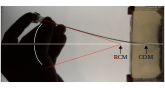
\includegraphics[width=0.65\columnwidth]{figures/rcm/rcm_vs_com.png}
  \caption{Needle base translation and rotation naturally forms a (virtual) remote center of motion (RCM), yet due to inherent flexibility of the partially embedded needle, needle deforms and forms a separate center of motion (COM). Without interaction with soft tissue, these two centers coincide.}
  \label{fig:rcm-vs-com}
\end{figure}

Yet the notion of an RCM is not completely irrelevant to needle-based procedures. For image-guided spinal injections, when a needle is misplaced, physicians would adjust the inserted needle by bending and laterally translating the needle base, and with the help of the reactive force generated by the soft tissue, they are able to pivot the needle tip onto a better trajectory~\parencite{fritzAugmentedRealityVisualization2012}. Such needle maneuver will not affect the target locations, which are encapsulated by the vertebrae. This needle manipulation roughly resembles a needle base rotational motion about a remote center, and the presence of a virtual RCM can be presumed, albeit at an unspecified location.

As an initial attempt to study the effect of this freehand needle manipulation and evaluate the possibility of enabling this motion on a robotic device in a safe manner, this chapter 1) parameterizes and replicates such motion by introducing a virtual RCM constraint to our existing platform, 2) models and examines the needle deflection profile in a tissue phantom, 3) introduces the notion of needle instant center of motion (COM), and 4) evaluates robot motion parameters that affect force variations during this \textit{in situ} needle motion.

\section{Materials and Methods}
\label{sec:chap-2-material-and-methods}

\subsection{System Overview}
\label{sec:chap-2-system-overview}

\begin{figure}[h]
  \centering
  \includegraphics[width = \columnwidth]{manuscripts/IROS_2021/figures/robot.eps}
  \caption{Overview of the PainBot system. The 4-DOF needle alignment module is attached to the cadaver torso. The 2-DOF needle driver module inserts and orients the needle based on manual inputs at the actuation unit. Image adapted from~\parencite{liFullyActuatedBodyMounted2020} with permission.}
  \label{fig:painbot_overview}
\end{figure}

As detailed in~\parencite{liFullyActuatedBodyMounted2020a,liFullyActuatedBodyMounted2020} and shown in~\cref{fig:painbot_overview} and ~\cref{fig:robot_kinematics}, PainBot is an MR-Conditional, body-mounted robotic device that can be used for MRI-guided lumbar injection procedures. Its 4-DOF needle alignment module assumes a straight-line needle trajectory between the target and entry points selected from pre-operative images, and aligns the needle driver module to the correct pose. Manual insertion is then performed remotely by the clinician by turning the crank of the actuation unit, which actuates the needle driver module via a beaded chain transmission mechanism. Needle longitudinal orientation could be changed by rotating the knob of the actuation unit, providing some needle steering capability.

A limitation in our previous clinical studies was the unmodeled needle-tissue behavior and the lack of direct haptic feedback. In particular, for facet joint injections, the needle often gets stuck inside of the fibrous tissue surrounding the joint capsule, in which case the clinician cannot successfully manipulate the needle using the two degrees of freedom provided by the needle driver; the only recourse is to retract the needle completely outside of the body and replan the trajectory, which prolongs the procedure and does not guarantee success in the following attempt.

In freehand insertion procedures, clinicians would tilt and translate the needle in order to correct the misplaced needle tip~\parencite{fritzAugmentedRealityVisualization2012}. This motion largely ensembles needle rotation around a fixed point in 3D space, i.e. a motion constrained by a virtual RCM. By choosing different locations for this virtual RCM, various needle deflections could be achieved, resulting in different degrees of tissue compression and needle tip displacements.


\subsection{Kinematics of Virtual RCM}
\label{sec:chap-2-kinematics}

As shown in~\cref{fig:robot_kinematics}, PainBot's top and bottom stage positions and their projections onto the vertical line, which goes through the virtual RCM point, form a pair of similar triangles $\triangle P_{t}O_{t}P_{rcm} \sim \triangle P_{b}O_{b}P_{rcm}$, and the vertical needle insertion depth $l = \| P_t - P_n \|_2 \cos{\theta}$ should be constant. Therefore, given a top stage position $P_t$ and the virtual RCM position $P_{rcm}$, the bottom stage position $P_b$ and needle tip position $P_n$ are readily calculated:
\begin{align}
  P_b & = \frac{P_{rcm} - P_{t}}{\| P_{rcm} - P_t \|_2} \frac{\| O_t - O_b \|_2}{\cos{\theta}} + O_t, \\
  P_n & = \frac{P_{rcm} - P_{t}}{\| P_{rcm} - P_t \|_2} \frac{l}{\cos{\theta}} + P_t.
\end{align}

The velocity of different components can be found by taking time derivatives of their geometric relations. Given an instantaneous top stage velocity $\vec{v}_t$,
\begin{align}
  \vec{v}_b &= \frac{\|P_b - P_{rcm}\|_2}{\|P_t - P_{rcm}\|_2} \vec{v}_t,\\
  \|\vec{v}_{in}\|_2 &= \frac{\|P_t - O_t\|_2}{\sqrt{\|P_t - O_t\|_2^2 + \|O_t - P_{rcm}\|_2^2}} \|\vec{v}_t\|_2,\\
  \dot\theta &= \frac{\cos^2{\theta}}{\|O_t - P_{rcm}\|_2} \|\vec{v}_t\|_2.
\end{align}



\begin{figure}[t]
  \centering
  \includegraphics[width = 0.65\columnwidth]{manuscripts/IROS_2021/figures/robot_kinematics_lettered.eps}
  \caption{Robot kinematics based on virtual RCM constraint. The needle (red) goes through the center of top and bottom stages of the needle alignment module. Current top and bottom stage positions ($P_{t}$ and $P_{b}$), and their projections ($O_{t}$ and $O_{b}$) with respect to the vertical line from the virtual RCM point ($P_{rcm}$), form a pair of similar triangles. An instantaneous change of position of the top stage ($\vec{v}_{t}$) will cause an instantaneous change of position of the bottom stage ($\vec{v}_{b}$) and of the needle ($\vec{v}_{in}$). Image adapted from~\parencite{liFullyActuatedBodyMounted2020a} with permission.}
  \label{fig:robot_kinematics}
\end{figure}

\subsection{Control Implementation}
\label{sec:chap-2-control-implementation}

As detailed in~\parencite{liFullyActuatedBodyMounted2020a}, the robot control software is based on MATLAB, where a custom software interface was designed to communicate with the embedded motion controller (DMC 4183, Galil Motion Control, USA) via serial communication. However, after the connection to the motion controller is established, the main MATLAB program runs only at about 5 Hz due to inadequate performance of MATLAB serial communication. Although this was not a requirement in~\cite{liFullyActuatedBodyMounted2020a}, the frequency is too low for responsive position tracking. To overcome this limitation, a mid-level controller is built using ROS Melodic and the Orocos Real-Time Toolkit (RTT). For position control, the main MATLAB program uploads relevant information (such as virtual RCM position) to a ROS parameter server; the mid-level controller retrieves these parameters and updates motor positions via the Galil Communication Library (gclib, Galil Motion Control, USA) at 100 Hz.

External input, such as digital signals from a joystick controller, is supported. The main MATLAB program takes in the external input as a top stage velocity command $\vec{v}_t$ in order to generate a smooth motion, and relays the command directly to the motion controller. The mid-level controller then tracks the bottom stage and needle insertion based on the top stage position. The external input is also able to change the virtual RCM location and desired motor speeds, as well as independently control the 2-DOF needle insertion module, allowing the operator to have full control over the robot for the virtual RCM manipulation. Note that top stage velocity $\vec{v}_t$ is preferred over bottom stage velocity $\vec{v}_b$ as input signal, since as long as the virtual RCM is positioned below the bottom stage, specifying a correct $\vec{v}_t$ will ensure that all motors operate within their speed limits.

\subsection{Preliminary Needle-Tissue Interaction Model}
\label{sec:chap-2-preliminary-interaction-model}

\begin{figure*}[t]
  \centering
  \includegraphics[width = \textwidth]{figures/rcm/needle_tissue_rcm.png}
  \caption{A planar view of virtual RCM motion of a needle inserted into an $N$-layer medium. The top and bottom stage displacements enforce the virtual RCM constraint ($m_2$ and $k_b$). The needle displaces the medium, generating an unknown reactive force distribution $F(x)$, which consists of normal force and friction force exerted by the medium. The mediums are modeled as a parallel arrangement of virtual springs, each with spring constants $k_i$ and friction coefficients $\gamma_i$. Along the inserted depth $l$, each spring is attached at end node of needle segment of length $l/n$. The reactive force deflects the needle to some shape $u(x)$, and causing the needle to intersect the $x$-axis at the instant center of motion (COM) where zero net displacement occurs.}
  \label{fig:needle_tissue_rcm}
\end{figure*}

A mathematical model is desired to understand how the needle interacts with the tissue during the virtual RCM motion. Although it has been established that biological soft tissues are nonlinear, anisotropic, fibrous composites~\parencite{petersonBiomechanicsPrinciplesApplications2007}, an idealized and linearized mechanics-based model is proposed to provide insights on how different parameters could qualitatively affect the the needle during the virtual RCM motion framework.

This preliminary model builds on a variation of the virtual spring approach which models the needle-tissue interaction as a linear beam supported by virtual springs~\parencite{glozmanImageGuidedRoboticFlexible2007,lehmannDeflectionModelingNeedle2017}. Considering small motion amplitudes and velocities, it is assumed that the virtual springs deflect within their linear elastic region, and viscous behavior is negligible. Without loss of generality, multiple types of springs can be incorporated in this model, each with spring constant $k_i$.
During the virtual RCM motion, the needle needs to be inserted or retracted to keep the RCM constraint, therefore friction between the outer surface of the needle cannula and the tissue is present. The friction force is discretized to be concentrated at each spring attachment location, and the friction force is modeled as proportional to the normal force exerted at that point, with coefficient of friction $\gamma_i$.

Taking a planar view of the needle lying horizontally, as shown in~\cref{fig:needle_tissue_rcm}, the needle deflection $v(x)$ is prescribed at the bottom stage. In addition, the virtual RCM constraint prescribes the incident slope at which the needle extends from the bottom stage. From the point of insertion to the needle tip, the needle cannula experiences axial forces by the deformed tissue, and also longitudinal forces caused by friction. Needle bending moment at the tip is taken as zero, and the needle tip's bevel shape is not taken into account.

To solve for the needle deflection, system total potential energy is first formulated. Rayleigh-Ritz method is then used to find a candidate polynomial that satisfies all the boundary conditions. Finally, the principle of minimum potential energy is invoked to find the remaining constant coefficients in the candidate function, thus giving us the deflection function that extremizes system potential energy. 

The total potential energy of the system is
\begin{equation}
  \Pi = (U_n + U_t) - WP_f,
\end{equation}
where $U_n$ is the strain energy in the needle caused by needle deflection, $U_t$ is the energy stored in the surrounding tissue due to elastic deformation, and $WP_f$ is the work potential of frictional force along the cannula surface.

More specifically, based on the Euler-Bernoulli beam theory,
\begin{equation}
  U_n = \int_{-s_b}^l{\frac{1}{2} EI \left(\frac{d^2u}{dx^2}\right)^2} dx,
\end{equation}
where $E$ and $I$ are the needle Young's modulus and area moment of inertia with respect to the axis of deflection.

Let $x_i = \frac{il}{n}$ be the $x-$coordinate of end node of the $i$th segment, then
\begin{equation}
  U_t = \sum_{i = 0}^{\left\lfloor n \right\rfloor} \frac{1}{2}k(x_i)u^2(x_i),
\end{equation}
where $k(x_i)$ is the linear elastic spring constant for a specific material at $x_i$, and $v(x_i)$ is the vertical displacement where $k_i$ is attached. 

Similarly
\begin{equation}
  WP_f = \sum_{i = 0}^{\left\lfloor n \right\rfloor} \gamma(x_i)k(x_i) u(x_i) \left( \sqrt{u^2(x_i) + \left(\frac{l}{n}\right)^2} - \left(\frac{l}{n}\right)\right).
\end{equation}

Notice that if $n \to \inf$, $\left(\frac{l}{n} \right) \to 0$, and $WP_f$ is simply
\begin{equation}
  WP_f \approx \sum_{i = 0}^{\left\lfloor n \right\rfloor} \gamma(x_i) k(x_i) u^2(x_i).
  \label{eq:virtual_work}
\end{equation}

When the number of finite elements, $\left\lfloor n\right\rfloor$, gets smaller, the length of each element, $l/n$, gets bigger, and $WP_f$ goes to zero; to best capture the interaction between the needle and tissue using the above model, the virtual work is expression is kept as in~\cref{eq:virtual_work}.

Unlike needle insertion path planning problems where the needle shape is completely unknown, the needle deflection expected in this local needle manipulation problem can be reduced to a beam bending problem, which can be adequately approximated by polynomial functions. An $r$th-order ($r \geq 3$) polynomial can be selected as the deflection candidate function which satisfies all boundary conditions:
\begin{align}
  &u(x)= \sum_{j=0}^r C_j x^j,\\
  &u(x = -s_b)= m_2, \\
  &\frac{du}{dx}\biggr\rvert_{x=-s_b}= k_b, \\
  &\frac{d^2u}{dx^2}\biggr\rvert_{x=l}= 0,
\end{align}
where the first two boundary conditions come from the virtual RCM constraint, while the third results from the assumption that the bending moment at the needle tip is negligible.

By requiring this form of $u$ to satisfy the boundary conditions, $u = u(x, C_r, C_{r-1}, \cdots, C_3)$. This expression can then be substituted into each of $U$ and $WP$ expressions such that $\Pi = \Pi(C_r, C_{r-1}, \cdots, C_3)$.

From the principle of minimum potential energy, the variation of $\Pi$ is zero, i.e.
\begin{equation}
  \delta\Pi = \delta\Pi(C_r, C_{r-1}, \cdots, C_3) = \sum_{p=3}^{r} \frac{\partial\Pi}{\partial C_p}\delta C_p= 0,
\end{equation}
and since $\delta C_p$ is arbitrary $\forall p$,
\begin{equation}
  \frac{\partial\Pi}{\partial C_p} = 0 \;\; \forall p.
\end{equation}

By completing the partial derivatives, the coefficients can be obtained by solving the system of linear equations and $v(x)$ can be readily calculated. This model is used to simulate the needle deflection for the virtual RCM motion, and the simulation result is presented in~\cref{sec:chap-2-simulation-and-parameter-identification}.

\section{Results} 
\label{sec:chap-2-results}

\subsection{Virtual RCM Implementation} 
\label{sec:chap-2-virtual-rcm-implementation}

% \begin{figure}[tb]
%   \centering
%   \includegraphics[width = \columnwidth]{figures/rcm_freespace_overlay.png}
%   \caption{Snapshots of the robot producing an RCM motion in sagittal plane, where the virtual RCM point is chosen to be at the needle tip.}
%   \label{fig:rcm_freespace}
% \end{figure}

A mid-level controller is implemented to achieve position control during the virtual RCM motion, and various motion parameters can be changed via an external joystick controller to achieve different needle trajectories. Due to the vibration generated by the ultrasonic motors, vibratory response of the needle driver and the attached needle makes it difficult to report reliable accuracy data of the virtual RCM motion using an optical tracking device; however, since no modification is done on the robot, and the virtual RCM constraint is maintained via position control, we have confidence to believe that the free space positioning accuracy is the same as reported in~\parencite{liFullyActuatedBodyMounted2020a}, which determined that the mean absolute errors of the tip position to be $0.99 \pm 0.46$ mm.

\subsection{COM Locations and Force Variations} 
\label{sec:chap-2-com-and-force}
As mentioned in~\parencite{fritzAugmentedRealityVisualization2012}, the average length of needle path for lumbar spinal injection procedures is $36.7\pm9.9$ mm. For the experiment, an insertion depth of $40$ mm is deemed sufficiently close to the clinical report. Of particular interest is how the location of the virtual RCM and tissue property will affect the needle deflection, as well as force variation, during the motion. Therefore, five virtual RCM points are chosen, whose locations are defined based on the needle insertion depth:

\begin{itemize}
  \item $0$ mm --- skin level
  \item $20$ mm --- $1/2$ insertion depth
  \item $40$ mm --- needle tip
  \item $60$ mm --- $3/2$ insertion depth
  \item $80$ mm --- 2 insertion depths
\end{itemize}

A 20 G$\times$20 cm Chiba biopsy needle (DCHN-20-20.0, Cook Medical, USA) is inserted straight into the gel phantoms, with bottom stage and gel top surface separation distance of $s_b = 27$ mm. Two single-layer gel phantoms with Shore OO hardness readings of 34 and 41 (X.F Durometer, Keyu, China) are used in the study. The robot is programmed to perform a back-and-forth virtual RCM motion in the sagittal plane to a designated maximum angulation limit, starting and finishing at the neutral vertical position. Other variables and their values are:

\begin{itemize}
  \item Top stage linear speed: [1.0, 1.5, 2.0, 2.5] mm/s
  \item Angulation limit about the vertical axis: [5.0, 7.5, 10.0] $^\circ$
\end{itemize}


Note that any two of the following quantities: virtual RCM location vRCM, bottom stage displacement $m_2$, and the needle incident angle $\theta$, determine the third, so any two variables could have been chosen as independent. Here, we decided that angulation is a more intuitive choice for the clinician during the operation, along with the virtual RCM position -- our main variable of interest, so they are chosen as the independent variables. Hence, a deeper RCM placement with the same angulation will necessarily result in a greater linear displacement of the bottom stage.

\begin{figure}[h]
  \centering
  \includegraphics[width = \columnwidth]{manuscripts/IROS_2021/figures/COM_comparison_lettered.eps}
  \caption{COM locations as a result of needle-tissue interaction during virtual RCM motion. Gel phantoms of Shore OO hardness 34 \textit{(left)} and 41 \textit{(right)} are used. Five different RCM locations are (a) $0.0$ mm, (b) $20.0$ mm, (c) $40.0$ mm, (d) $60.0$ mm, and (e) $80.0$ mm underneath the gel top surface (red line). Physical distance between the gel top surface and needle tip is $40.0$ mm. The needle COM regions are marked in white, with green dots indicating the approximated COM points.}
  \label{fig:com_compare}
\end{figure}

The needle COM regions are captured according to~\cref{sec:chap-2-com-and-force}, and the results for the two types of gel phantoms are presented in~\cref{fig:com_compare}. The green dots indicate the depths of COM points of the needle across the five virtual RCM locations and between the two gels. Experimentally found COM locations can be found in~\cref{tab:COM_pos_table}.


\begin{table}[h]
\centering
\caption{Experimentally determined COM locations, $E_{com}$, and simulated COM locations, $S_{com}$, for the two gel materials.}
\resizebox{0.5\columnwidth}{!}{%
\begin{tabular}{|c|c|c|c|c|c|}
\hline
vRCM (mm)                             & \textbf{0}                & \textbf{20}               & \textbf{40}               & \textbf{60}               & \textbf{80}               \\ \hline
34 $E_{com}$ (mm)                       & 21.3                      & 26.1                      & 27.7                      & 28.3                      & 28.4                      \\ \hline
34 $S_{com}$ (mm)                       & 21.2                      & 26.7                      & 27.6                      & 28.0                      & 28.3                      \\ \hline
\multicolumn{1}{|l|}{41 $E_{com}$ (mm)} & \multicolumn{1}{l|}{22.8} & \multicolumn{1}{l|}{25.2} & \multicolumn{1}{l|}{26.0} & \multicolumn{1}{l|}{26.9} & \multicolumn{1}{l|}{26.9} \\ \hline
\multicolumn{1}{|l|}{41 $S_{com}$ (mm)} & \multicolumn{1}{l|}{22.7} & \multicolumn{1}{l|}{25.8} & \multicolumn{1}{l|}{26.3} & \multicolumn{1}{l|}{26.5} & \multicolumn{1}{l|}{26.6} \\ \hline
\end{tabular}%
}
\label{tab:COM_pos_table}
\end{table}

As shown in the figure, the COM point gets lower as the virtual RCM location lowers, but at a decreasing rate. Material hardness also dictates the behavior, as the COM points for the softer material tend to spread out more, indicating a greater efficacy of the virtual RCM approach on softer tissues than on harder ones. The diminishing value of lowering the virtual RCM point also suggests that there is a fundamental limit imposed by the tissue of the amount of control we have over the needle once it is inserted into the tissue.

Force data are collected via a 6-axis F/T sensor at the bottom of the testbed, and reflect the net force transmitted from the gel to the sensor. Different insertion configurations will result in different durations to complete the back-and-forth motion, therefore the data are rescaled in time to represent force at different stages of the motion. For example, data when the motion at $-\theta_{max}$ completed correspond to the needle driver situated at its far left position; data at $\theta_{max}$ correspond to the far right position.

For a $1.5$ mm/s top stage linear motion speed and a $5^\circ$ maximum angulation limit, the net force is greater for the harder gel than it is for the softer gel, as shown in~\cref{fig:material_rcm_compare}. Comparing the two plots suggests that given the same type of RCM motion, a softer tissue will more readily resolve needle compression force into local tissue deformation, thus allowing smaller net force to be transmitted to the surrounding tissue; harder tissue offers less room for local deformation, and the load from the needle is shared by the surrounding tissue at a greater vicinity.

\begin{figure}[tb]
  \centering
  \includegraphics[width = \columnwidth]{manuscripts/IROS_2021/figures/material_rcm_compare_relabeled.png}
  \caption{Force data for $1.5$mm/s top stage linear speed and up to $5^\circ$ angulation inside of two gels. Virtual RCM position varies from skin level to twice the insertion depth.}
  \label{fig:material_rcm_compare}
\end{figure}

Analogous to a clinician's hand movement speed, the top stage linear motion speed is another independent variable in the study. However, in the present experiment, speed does not affect the net force; rather, how fast it reaches its peak value. As shown in~\cref{fig:speed_angle_compare}, the net forces across different speeds remain very close to each other, with maximum force difference of approximately $0.02$ N. It is also not surprising to observe that a greater angulation will generate greater net force, since the gel will be displaced to a greater extent.

\begin{figure}[tb]
  \centering
  \includegraphics[width = \columnwidth]{manuscripts/IROS_2021/figures/speed_angle_compare_relabeled.png}
  \caption{Force data for 34 Shore OO hardness reading gel and $40$ mm virtual RCM placement with two angulation limits. Speed varies from $1.0$ mm/s to $2.5$ mm/s.}
  \label{fig:speed_angle_compare}
\end{figure}

Force data asymmetry is a result of an eccentric sensor-needle alignment, which causes a higher reading in the direction of offset. In this particular set of data, the needle is positioned slightly onto the positive $x-$axis, causing a higher force reading during the second half of the motion than the first. Although it does not obscure our findings, this data asymmetry will be removed from using a better setup.

\subsection{Model Simulation and Parameter Identification}
\label{sec:chap-2-simulation-and-parameter-identification}
Simulations are carried out to validate the mathematical model, as well as identifying parameter values that match the simulation with the experimental result. The needle is made out of material similar to A304 stainless steal, which has a nominal Young's modulus of $E = 190$ GPa. The area moment of inertia of the 20 G needle cannula and inner stylet is $I = 0.027$ mm$^4$.

A $3rd$-order polynomial is chosen to be the candidate function for applying the Rayleigh-Ritz method, and the solutions are arrived according to~\cref{sec:chap-2-preliminary-interaction-model}. Although it is possible to select a higher-order polynomial, overfitting could deviate the model further from reality.

According to~\parencite{urreaEvaluationFrictionCoefficient2016}, the average dynamic coefficient of friction between the surface of A304 stainless steel needle and that of an agarose hydrogels is found to be 0.255, which is taken to be the value of $\mu$. The other two variables, $k$ and $n$, are found iteratively via a nonlinear minimization algorithm such that
\begin{equation}
  \left\{k, n\right\} = \argmin {\|S_{com} - E_{com}\|_2},
\end{equation}
where $S_{com}$ is a vector of simulated COM positions, and $E_{com}$ is a vector of experimental COM positions found in~\cref{sec:chap-2-com-and-force}.

By minimizing the COM differences across all five virtual RCM locations, the parameter values for the gel phantom with 34 Shore OO hardness reading is $k_{34} = 1.6889$ N/m and $n_{34} = 1.1840$, while $k_{41} = 4.1484$ N/m with $n_{41} = 2.1977$ for the 41 Shore OO hardness gel. Normed differences between $E_{com}$ and $S_{com}$ are $0.72$ mm and $0.82$ mm, respectively. Simulated needle shapes are shown in Figure~\ref{fig:T1T2_sim}, and the corresponding simulated COM points are reported in~\cref{tab:COM_pos_table}.

Note that a non-integer $n$ implies that there are $(\lfloor n \rfloor + 1)$ linear springs attached $l/n$ apart from each other along the needle, with the first spring attached at the top gel surface where the needle first contacts the gel.

\begin{figure}[tb]
  \centering
  \includegraphics[width = \columnwidth]{figures/rcm/T1T2_sim.png}
  \caption{Simulation of the proposed needle-tissue interaction model with fixed $m_2 = 10$. Needle deflection with five different virtual RCM locations are compared when the needle is inserted into two types of tissues. The virtual RCM locations are marked in circles, and the corresponding needle deflection shapes are plotted in the same color. The instant COM points are the intersections of the needle shape with the $x$-axis.}
  \label{fig:T1T2_sim}
\end{figure}

The mathematical model, along with the parameter values returned by the minimization algorithm, agrees with the experimental results in that a harder gel requires more virtual springs with higher spring constants to be attached on the needle. With sufficient knowledge of the material properties, the model should be able to predict the behavior of the needle to sub-millimeter accuracy across the whole spectrum of virtual RCM selections, given that the tissue displacement stays within its linear elastic range.

If the virtual RCM point is placed infinitely deep, the resulting needle motion resembles a pure lateral translation where little to no tilting is involved. With certain set of needle and tissue properties, pure needle translation will not generate a physical COM point on the needle; rather, the needle tip translates in the same direction as does the rest of the needle. However, the net tissue displacement for pure needle translation can be larger than necessary.

Consider the case presented in~\cref{fig:trans_vs_com}. A needle tip relocation is needed during a surgical procedure, and the desired needle tip displacement is $-5$ mm in the $y-$direction. For this tissue, it is found that a pure translational needle motion of  $10$ mm is sufficient to bring the needle tip to the desired location; however, with a virtual RCM placed at $9.81$ mm underneath the skin, the same base displacement in the opposite direction will achieve the same result, with a COM at $15.09$ mm. The net tissue displacement can be represented by the absolute area between the needle deflection curve and its initial position, i.e.
\begin{equation}
  A_{tissue} = \int_0^{l}{|v(x)|}dx.
\end{equation}
For the pure translational motion, $A_{trans} = 287.44$ mm$^2$, while $A_{com} = 89.15$ mm$^2$ for the virtual RCM motion, which is less than its non-COM-inducing counterpart. With less amount of tissue displacement, the risk of tissue damage during needle tip relocation for the virtual RCM motion is lowered.

\begin{figure}[h]
  \centering
  \includegraphics[width = \columnwidth]{manuscripts/IROS_2021/figures/translation_vs_RCM.png}
  \caption{A simulated example comparing pure needle translation and COM-inducing virtual RCM motion to achieve the same needle tip relocation.}
  \label{fig:trans_vs_com}
\end{figure}

\section{Discussion} 
\label{sec:chap-2-discussion-and-conclusion}
Remote center of motion is commonly used in medical robotics for minimally invasive procedures; however, the implication between having an RCM and ``minimally invasive'' is subtle and highly dependent on the nature of the medical procedure. This paper has shown that for a flexible needle that has been inserted into the tissue, a virtual RCM is not the best indicator of a safe \textit{in situ} needle manipulation; rather, it is the needle center of motion --- COM --- that provides this information. 

As the point of zero net displacement, the needle COM can be positioned at certain anatomically critical location, and can ensure minimal deformation of the surrounding tissue during some necessary needle relocation maneuvers. Being the ``fulcrum'' where the needle rotates, the COM can ensure the overall tissue displacement to be small, such as the example presented in~\cref{fig:trans_vs_com}. By selectively placing the virtual RCM robot constraint, one can tune the behavior of the needle and tissue reactions, and use the COM to one's advantage for a safe \textit{in situ} needle manipulation.

However, the experiments and simulations have shown that it is up to the surrounding tissue to decide whether the needle can be brought to a desired state with a virtual RCM motion. With the needle inserted deep into a hard tissue, the efficacy of the virtual RCM approach quickly diminishes, and the best course of action is likely to be retracting the needle to a shallower depth, where less amount of tissue is there to resist needle motion. The method of optimally positioning this needle COM by way of choosing a robot virtual RCM will be investigated in the future. Force data can be compared when a clinician performs the same task using freehand technique to further evaluate the safety of the proposed needle manipulation method.

A few sources of error should be addressed, and some should be eliminated during subsequent studies. In terms of the experiment setup, the portable PainBot platform forbids excessive modification on the robotic system itself, thus a temporary setup was made to conduct the experiments, and data accuracy is limited. The force sensor used in the study has sensing range up to $125$ N in the $x-$ and $y-$direction, and up to $500$ N in the $z-$direction, while the forces involved in the experiments reside in the far smaller range. A series of noise attenuations were performed before force data are compared, but a better choice of force sensor could improve data resolution. A dedicated camera could be installed to capture higher quality images and videos to make it easier for needle shape detection during the RCM motion, and parameter identification can be done not only to match the simulated COM points, but also the final shape of the needle as well.

In terms of modeling, simplification was made for the method to yield a linear system of equations. Although the current model captures the nature of the needle-tissue interaction to a reasonable degree, real tissues will present much greater challenges, such as nonlinearity, viscosity, and rupture. Model validation will be performed when needle shape information is available, and the model will be tested in a combination of gels and real tissues. One important assumption is that the needle has no deflection prior to the virtual RCM motion --- this allows the virtual RCM to be positioned on the needle longitudinal axis. In situations where initial needle deflection exists, a needle shape approximation needs to be made first, but the choice of virtual RCM location will be less intuitive.

If an accurate model can be obtained in the lab environment, efforts will follow to further this research in an MRI facility, such as integrating fiber Bragg grating sensors into the needles for shape sensing, and building an MR-compatible joystick controller for virtual RCM robot control inside of the scanner room.

In conclusion, a robot virtual RCM constraint can induce a needle COM upon which the needle pivots in the tissue. For operations such as robot assisted lumbar injections, the induced COM can result in less tissue displacement than its non-COM-inducing counterparts for a desired needle relocation, thus presents a safer alternative for \textit{in situ} needle manipulations during the procedure.

\section{Chapter Acknowledgment}
\label{sec:chap-2-ack}

I would like to thank Dr. Karun Sharma for providing insight regarding safe \textit{in situ} needle manipulations, as well as agreeing to the recording of his hand motion that produced~\cref{fig:rcm-vs-com}.

%%% Local Variables:
%%% mode: LaTeX
%%% TeX-master: "main"
%%% End:
